\documentclass[12pt,notheorems,aspectratio=169,notes,handout]{beamer}
%%% single-line packages %%%
%%%%%%%%%%%%%%%%%%%%%%%%%%%%
\usepackage[utf8]{inputenc}
\usepackage{standalone}
%\usepackage{babel}% For multilingual/non-English documents.
%\usepackage{csquotes}% Load if you want non-English quotes.
%\usepackage{xpatch}% For some biblatex styles, this is required. Not for the core ones.
%\usepackage[backend=biber,style=alphabetic]{biblatex}% Biblatex+Biber setup. Your document will now take a while to compile.
%\usepackage{graphicx}

%%% Isabelle Listings %%%
%%%%%%%%%%%%%%%%%%%%%%%%%
\usepackage{lisa}% includes amssymb, fancyvrb, listings, xcolor, bigfoot, ltxcmds

%%% hyperref %%%
%%%%%%%%%%%%%%%%
\usepackage{hyperref}
% This colours the hyperlinks, which is better for screen reading. COMMENT for printing/colorblind-friendliness.
\hypersetup{
    colorlinks,
    linkcolor={red!50!black},
    citecolor={blue!50!black},
    urlcolor={blue!80!black}
}

%%% AMS packages %%%
%%%%%%%%%%%%%%%%%%%%
\usepackage{physics}% includes amsmath, great for \bra and \ket etc.
\usepackage{mathtools}
\usepackage{amsthm}
% additional symbol definitions
\newcommand\restr[2]{{% we make the whole thing an ordinary symbol
  \left.\kern-\nulldelimiterspace % automatically resize the bar with \right
  #1 % the function
  \vphantom{\big|} % pretend it's a little taller at normal size - comment if not wanted
  \right|_{#2} % this is the delimiter
}}

% Environment definitions, mostly standard
\theoremstyle{plain}% default
\newtheorem{theorem}{Theorem}[section]
\newtheorem{lemma}[theorem]{Lemma}
\newtheorem{proposition}[theorem]{Proposition}
\newtheorem*{corollary}{Corollary}

\theoremstyle{definition}
\newtheorem{definition}{Definition}[section]
\newtheorem{axiom}{Axiom}[section]
\newtheorem{example}{Example}[section]
\newtheorem{exercise}[example]{Exercise}

\theoremstyle{remark}
\newtheorem*{remark}{Remark}
%\newtheorem*{note}{Note} % Notes are already defined in beamer - I think for presentor mode?

% TODO look into the cleveref package and hyperref's \autoref
%%% fancyref %%%
%%%%%%%%%%%%%%%%
\usepackage[plain]{fancyref}% tight spacing because I use abbreviated cross references, e.g. Fig. 1
{%%% old format -- short, abbreviated names, grammatical capitalisation only, tight spacing %%%
%% new prefixes
%\newcommand*{\fancyrefthmlabelprefix}{thm}
%\newcommand*{\fancyrefdeflabelprefix}{def}
%\newcommand*{\fancyrefeqnlabelprefix}{eqn}
%\newcommand*{\fancyreflinelabelprefix}{line}
% spacing used in all commands, not just the ones (re)defined below
%\renewcommand*{\fancyrefdefaultspacing}{\fancyreftightspacing}
%% new names and formats
%\newcommand*{\Frefdefname}{Def.}
%\newcommand*{\frefdefname}{def.}
%\frefformat{plain}{\fancyrefdeflabelprefix}{\frefdefname\fancyrefdefaultspacing#1}
%\Frefformat{plain}{\fancyrefdeflabelprefix}{\Frefdefname\fancyrefdefaultspacing#1}
%\newcommand*{\Frefeqnname}{Eqn.}
%\newcommand*{\frefeqnname}{eqn.}
%\frefformat{plain}{\fancyrefeqnlabelprefix}{\frefeqnname\fancyrefdefaultspacing#1}
%\Frefformat{plain}{\fancyrefeqnlabelprefix}{\Frefeqnname\fancyrefdefaultspacing#1}
%\newcommand*{\Freflinename}{Line}
%\newcommand*{\freflinename}{line}
%\frefformat{plain}{\fancyreflinelabelprefix}{\freflinename\fancyrefloosespacing#1}
%\Frefformat{plain}{\fancyreflinelabelprefix}{\Freflinename\fancyrefloosespacing#1}
%% existing name (and format?) changes (here, shortened)
%%\renewcommand*{\Frefeqname}{Eqn.}
%\renewcommand*{\Frefsecname}{Sec.}
%\renewcommand*{\Freftabname}{Tab.}
%\renewcommand*{\Freffigname}{Fig.}
}
% new prefixes
\newcommand*{\fancyrefthmlabelprefix}{thm}
\newcommand*{\fancyreflemlabelprefix}{lem}
\newcommand*{\fancyrefapplabelprefix}{app}
\newcommand*{\fancyrefdeflabelprefix}{def}
\newcommand*{\fancyrefeqnlabelprefix}{eqn}
\newcommand*{\fancyreflinelabelprefix}{line}
% spacing used in all commands, not just the ones (re)defined below
\renewcommand*{\fancyrefdefaultspacing}{\fancyrefloosespacing}
% new names and formats
\newcommand*{\Frefdefname}{Definition}
\newcommand*{\frefdefname}{definition}
\frefformat{plain}{\fancyrefdeflabelprefix}{\frefdefname\fancyrefdefaultspacing#1}
\Frefformat{plain}{\fancyrefdeflabelprefix}{\Frefdefname\fancyrefdefaultspacing#1}
\newcommand*{\Frefappname}{Appendix}
\newcommand*{\frefappname}{appendix}
\frefformat{plain}{\fancyrefapplabelprefix}{\frefappname\fancyrefdefaultspacing#1}
\Frefformat{plain}{\fancyrefapplabelprefix}{\Frefappname\fancyrefdefaultspacing#1}
\newcommand*{\Frefeqnname}{Equation}
\newcommand*{\frefeqnname}{equation}
\frefformat{plain}{\fancyrefeqnlabelprefix}{\frefeqnname\fancyrefdefaultspacing#1}
\Frefformat{plain}{\fancyrefeqnlabelprefix}{\Frefeqnname\fancyrefdefaultspacing#1}
\newcommand*{\Freflemname}{Lemma}
\newcommand*{\freflemname}{lemma}
\frefformat{plain}{\fancyreflemlabelprefix}{\freflemname\fancyrefdefaultspacing#1}
\Frefformat{plain}{\fancyreflemlabelprefix}{\Freflemname\fancyrefdefaultspacing#1}
\newcommand*{\Frefthmname}{Theorem}
\newcommand*{\frefthmname}{theorem}
\frefformat{plain}{\fancyrefthmlabelprefix}{\frefthmname\fancyrefdefaultspacing#1}
\Frefformat{plain}{\fancyrefthmlabelprefix}{\Frefthmname\fancyrefdefaultspacing#1}
\newcommand*{\Freflinename}{Line}
\newcommand*{\freflinename}{line}
\frefformat{plain}{\fancyreflinelabelprefix}{\freflinename\fancyrefloosespacing#1}
\Frefformat{plain}{\fancyreflinelabelprefix}{\Freflinename\fancyrefloosespacing#1}
% existing name (and format?) changes (here, shortened)
%\renewcommand*{\Frefeqname}{Eqn.}
\renewcommand*{\Frefsecname}{Section}
\renewcommand*{\Freftabname}{Table}
\renewcommand*{\Freffigname}{Figure}
% Capitalise everything!
\renewcommand{\fref}{\Fref}

%%% TiKZ %%%
\usepackage{tikz}
%\usetikzlibrary{arrows}
\usetikzlibrary{cd}
\usetikzlibrary{decorations.pathreplacing,calc} % needed for braces across itemize (below)
\usetikzlibrary{tikzmark} % needed for drawing rectangles around highlights in lstlistings

%%% mathtools %%%
%%%%%%%%%%%%%%%%%
\usepackage{mathtools}
\DeclarePairedDelimiter{\all}{\forall}{.\quad}
\DeclarePairedDelimiter{\any}{\exists}{.\quad}
%%% strikeout in math mode
% from : https://tex.stackexchange.com/a/20613
\newcommand\hcancel[2][black]{\setbox0=\hbox{$#2$}%
\rlap{\raisebox{.45\ht0}{\textcolor{#1}{\rule{\wd0}{1pt}}}}#2}


%%% Symbol shortcuts and custom commands %%%
%%%%%%%%%%%%%%%%%%%%%%%%%%%%%%%%%%%%%%%%%%%%
\newcommand{\setN}{{\mathord{\mathbb N}}}
\newcommand{\setZ}{{\mathord{\mathbb Z}}}
\newcommand{\setQ}{{\mathord{\mathbb Q}}}
\newcommand{\setR}{{\mathord{\mathbb R}}}
\newcommand{\setC}{{\mathord{\mathbb C}}}
\newcommand{\setH}{{\mathord{\mathbb H}}}

\def\ie/{\textit{i}.\textit{e}.}
\def\eg/{\textit{e}.\textit{g}.}
\def\cf/{\textit{cf}.}

%%% Drawing rectangles to highlight parts of listings %%%
\newcounter{lstmark}
\newcommand{\tmark}[2][0pt]{%tikzmark
    \stepcounter{lstmark}%
    \if###2##%
    \else
        #2%
    \fi
    \tikz[overlay,remember picture]\node (\thelstmark){};%
}
\newcommand{\makehl}[3][0pt]{%make highlight
    \begin{tikzpicture}[overlay, remember picture]
        \draw[red,rounded corners]
          let \p1=(#2), \p2=(#3) in
          ({\x1-3pt}, {\y1+1.65ex})
            rectangle
          ({\x2+3pt}, {\y2-0.65ex});
    \end{tikzpicture}%
}

%%% Braces over multiple itemized items %%%
\newcounter{itemnum}
\newcommand{\nt}[2][0pt]{%
    \stepcounter{itemnum}%
    \if###2##%
    \else
        #2%
        \thinspace
    \fi
    \tikz[overlay,remember picture,baseline=(\theitemnum.base),xshift=#1]\node (\theitemnum){};%
}
\newcommand{\makebrace}[4][0pt]{%
    \begin{tikzpicture}[overlay, remember picture]
        \draw [decoration={brace,amplitude=0.5em},decorate]
        let \p1=(#2), \p2=(#3) in
        ({max(\x1+#1,\x2+#1)}, {\y1+1.75ex}) --
            node[right=0.6em] {#4} ({max(\x1+#1,\x2+#1)}, {\y2-0.5ex});
    \end{tikzpicture}%
}
\newenvironment{braceitems}{%
    \begin{enumerate}
}{%
    \end{enumerate}
    \setcounter{itemnum}{0}%
}


%%% single-line packages %%%
%%%%%%%%%%%%%%%%%%%%%%%%%%%%
\usepackage{setspace}% For adjusting spacing between lines\comment{text}{comment}

%%% Custom commands %%%
%%%%%%%%%%%%%%%%%%%%%%%

% Borderless frame for including big images
% TODO not well tested - may break some title bars or footers?
% TODO may also benefit from some more refinement over just setting all margins to 0
\newenvironment{emptyframe}
{
 % not too sure, but may be needed if you have a background image
 % that should not appear on this kind of frame:
 \setbeamertemplate{background canvas}[default]
 % turn off navigation symbols for this frame
 \setbeamertemplate{navigation symbols}{}
 % locally set margins to zero: (notice the use of \bgroup ... \egroup
 % to limit the scope of the geometry restriction
 % where curly brackets {} aren't possible)
 \bgroup \newgeometry{margin=0cm}
 \begin{frame}[plain]
}
{
 \end{frame}
 \egroup
}

% footnote without label, e.g. for same-slide references
\newcommand{\nolabelfootnote}[1]{%
  \begingroup
  \renewcommand{\thefootnote}{}
  \footnote[frame]{\hspace{-18pt}\tiny#1}%
  \addtocounter{footnote}{-1}%
  \endgroup
}

% Improved version of \alt. Keeps constant width to avoid jiggling slides.
% https://tex.stackexchange.com/questions/13793/beamer-alt-command-like-visible-instead-of-like-only
\makeatletter
% Detect mode. mathpalette is used to detect the used math style
\newcommand<>\Alt[2]{%
    \begingroup
    \ifmmode
        \expandafter\mathpalette
        \expandafter\math@Alt
    \else
        \expandafter\make@Alt
    \fi
    {{#1}{#2}{#3}}%
    \endgroup
}
% Un-brace the second argument (required because \mathpalette reads the three arguments as one
\newcommand\math@Alt[2]{\math@@Alt{#1}#2}
% Set the two arguments in boxes. The math style is given by #1. \m@th sets \mathsurround to 0.
\newcommand\math@@Alt[3]{%
    \setbox\z@ \hbox{$\m@th #1{#2}$}%
    \setbox\@ne\hbox{$\m@th #1{#3}$}%
    \@Alt
}
% Un-brace the argument
\newcommand\make@Alt[1]{\make@@Alt#1}
% Set the two arguments into normal boxes
\newcommand\make@@Alt[2]{%
    \sbox\z@ {#1}%
    \sbox\@ne{#2}%
    \@Alt
}
% Place one of the two boxes using \rlap and place a \phantom box with the maximum of the two boxes
\newcommand\@Alt[1]{%
    \alt#1%
        {\rlap{\usebox0}}%
        {\rlap{\usebox1}}%
    \setbox\tw@\null
    \ht\tw@\ifnum\ht\z@>\ht\@ne\ht\z@\else\ht\@ne\fi
    \dp\tw@\ifnum\dp\z@>\dp\@ne\dp\z@\else\dp\@ne\fi
    \wd\tw@\ifnum\wd\z@>\wd\@ne\wd\z@\else\wd\@ne\fi
    \box\tw@
}
\makeatother

%
% Choose how your presentation looks.
%
% For more themes, color themes and font themes, see:
% http://deic.uab.es/~iblanes/beamer_gallery/index_by_theme.html
%
\mode<presentation>
{
  \usetheme{default}      % or try Darmstadt, Madrid, Warsaw, ...
  \usecolortheme{default} % or try albatross, beaver, crane, beetle, seagull, dove, fly ...
  \usefonttheme{default}  % or try serif, structurebold, ...
  \setbeamertemplate{navigation symbols}{}
  \setbeamertemplate{caption}[numbered]
}

\title[]{%
  Haag-Kastler Nets in Isabelle/HOL\\%
  \normalsize{Formalising an Algebraic Approach to\\Quantum Field Theory}}
\author{Richard Schmoetten}
\institute{The University of Edinburgh}
\date{31st August 2022}

\begin{document}

\begin{frame}
  \titlepage
\end{frame}
\note{}

\begin{frame}{Testing the SM}
\begin{itemize}
	\item<1- > Fine structure constant $\alpha^{-1} = 137.035999084(21)$ CODATA
	\note[item]<1- >{
		related to the scale of EM interactions \\
		std uncertainty: $1.5 \times 10^{-10}$ \\
		measuring polar diameter to within $0.1$ hair's width!}
	\item<2- > Anomalous magnetic dipole of $\mathrm{e^-}$\nt{}
	\item<3- > Recoil frequency of Cesium-133\nt{}
	\note[item]<2- >{
    Fine structure constant is calculated from $g-2$  measurement and calculation of $>10000$ diagrams! No more dark photons ($2.5 \sigma$). Limited by $g_e -2$ accuracy.}
	\item<4-6> \alt<4>{In agreement...}{\alt<5>{Not in disagreement...}{Not in disagreement... As of just now!}}
  \note[item]<4- >{
    $<1\sigma$ tension with prior recoil measurement, $2.5\sigma$ tension with gyromag measurement. Fermilab (4/2021) brings this to $4.2\sigma$, on $g_{\mu}-2$.}
\end{itemize}
\begin{onlyenv}<4- >
  \vspace{-12pt}\makebrace[5pt]{1}{2}{compare}
\end{onlyenv}
\end{frame}

\begin{frame}{Quantum Field Theory}
  \begin{itemize}
    \item<1- > Framework for the different parts of the standard model.
    \item<2- > Based on the idea of path integrals.
    \item<3- > Many theoretical breakthroughs: renormalisation, QCD asymptotic freedom, Higgs boson, \dots
  \end{itemize}
  \vfill
  \begin{overlayarea}{\textwidth}{0.35\textheight}
    \only<2-3|handout:0>{
      \centering
      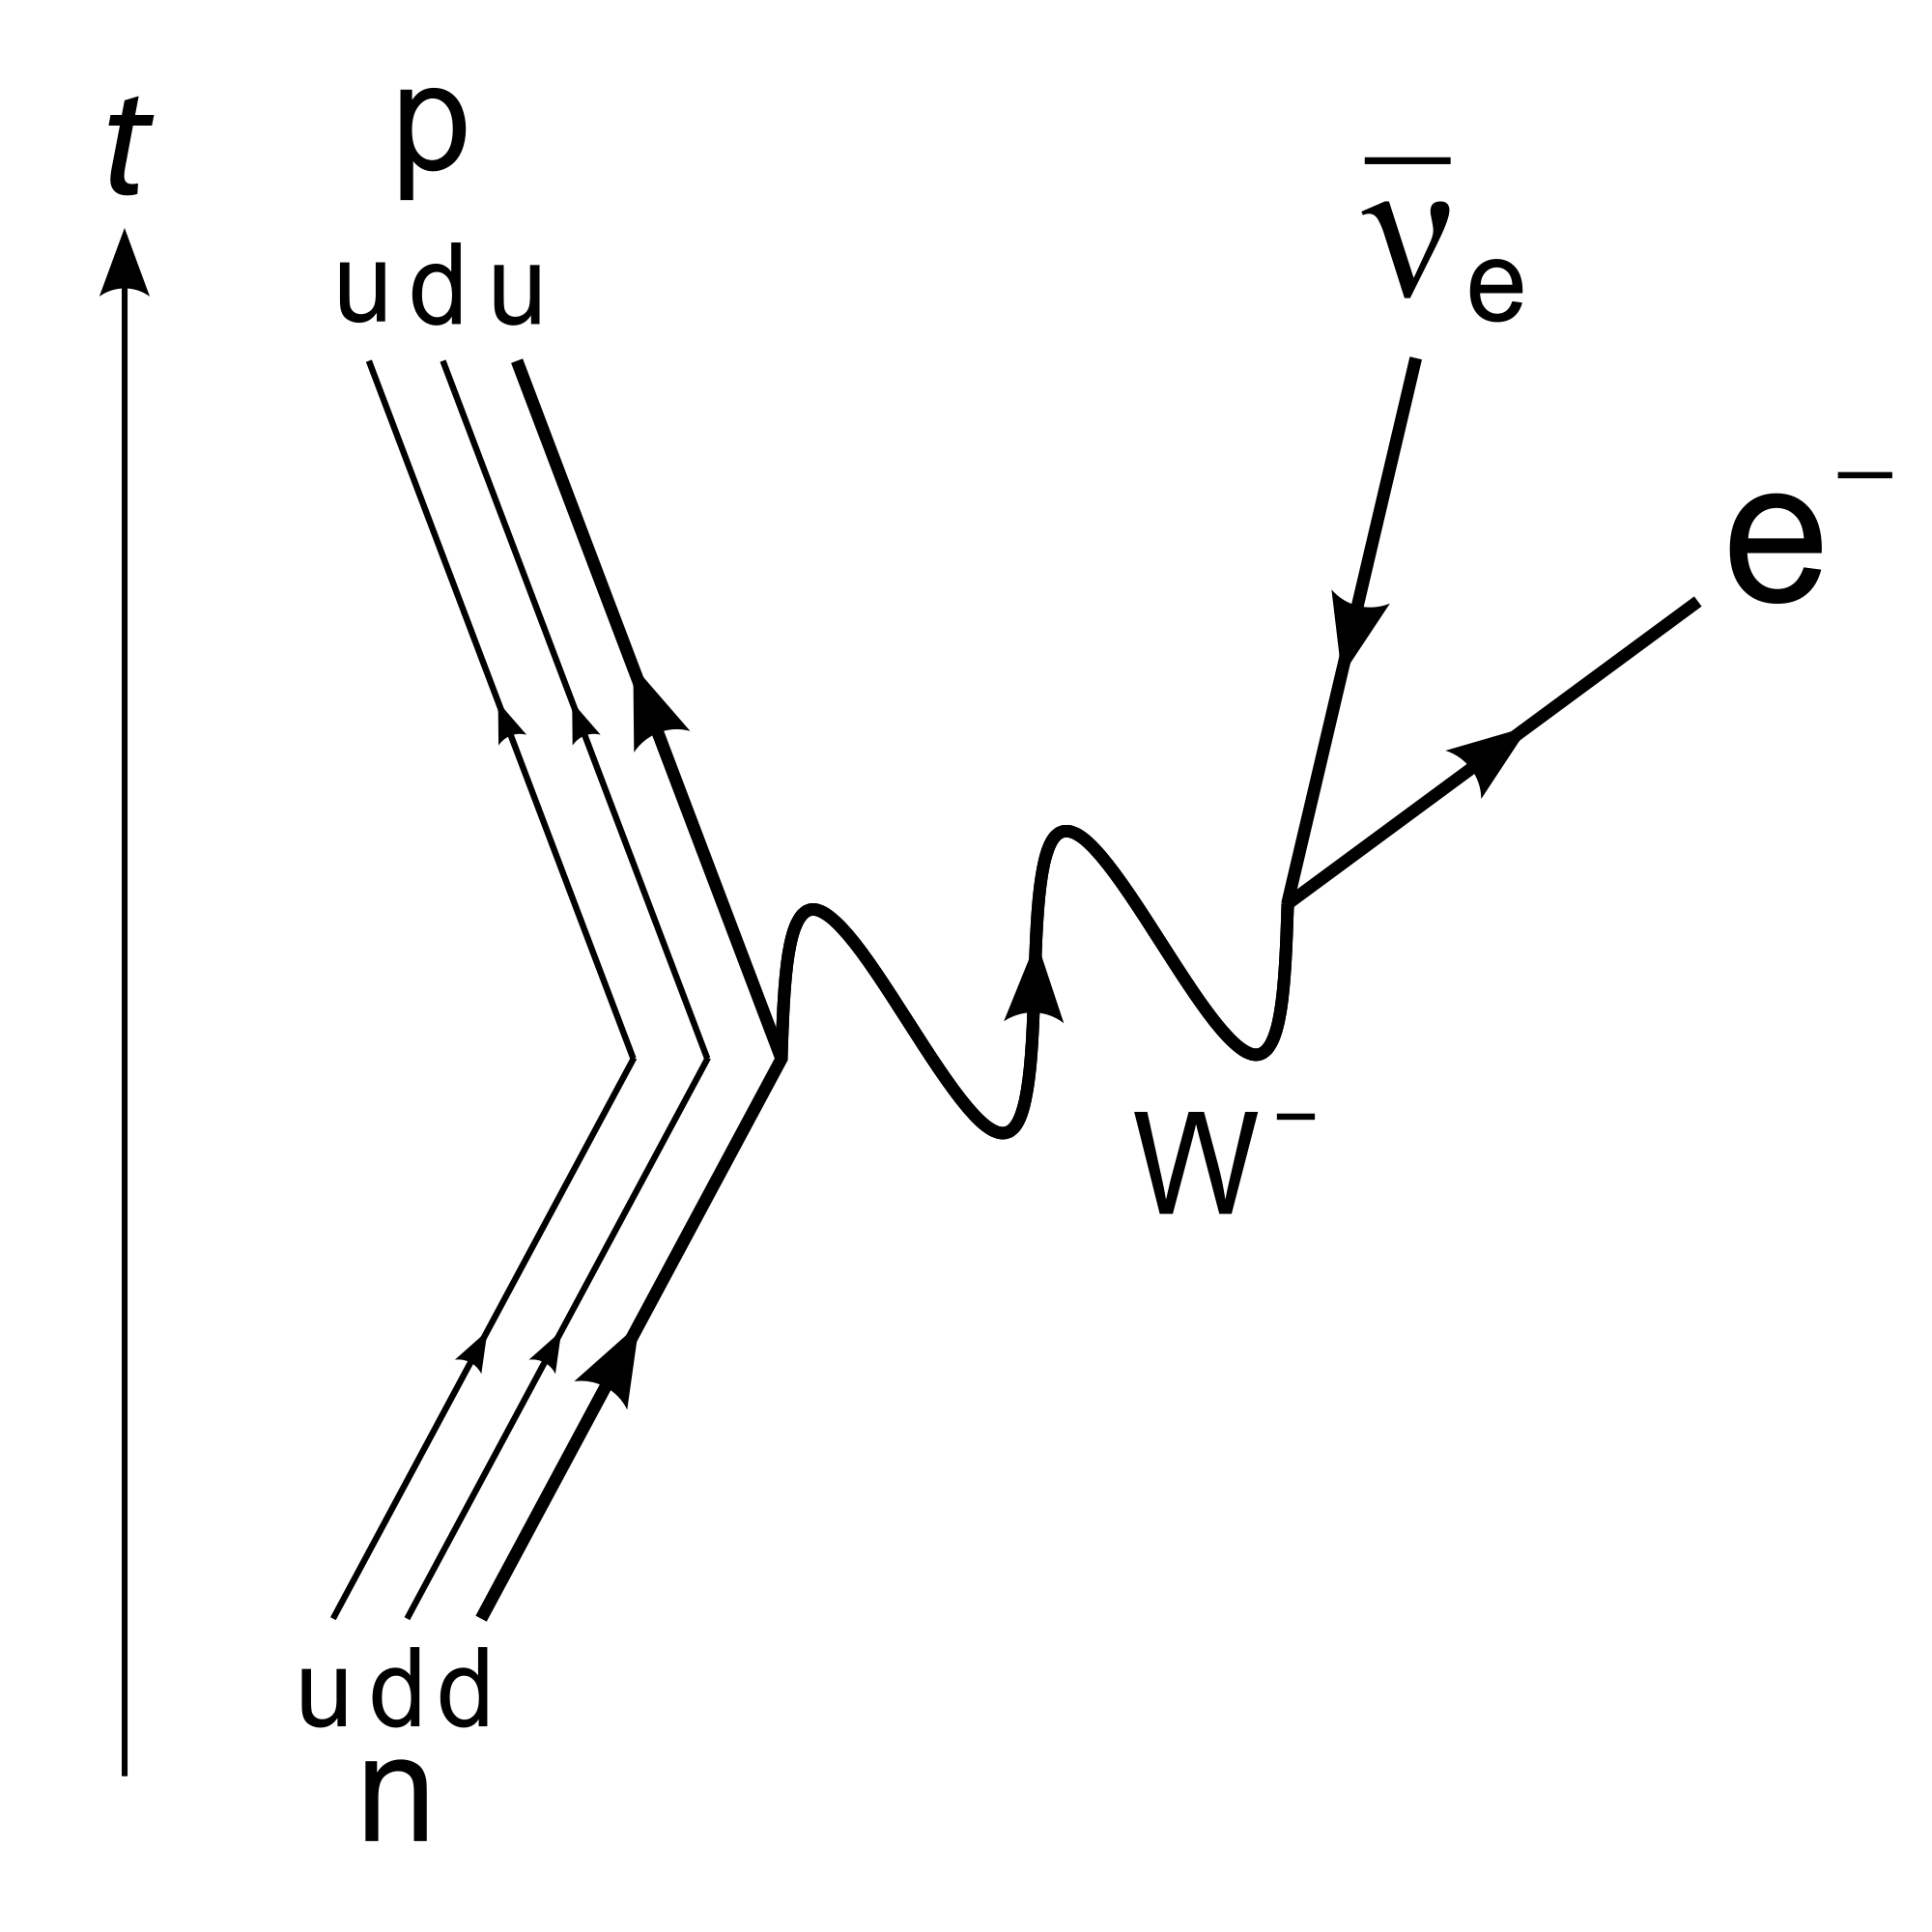
\includegraphics[width=0.25\linewidth]{feynman-diag-beta-decay.png}%
      \hspace{35pt}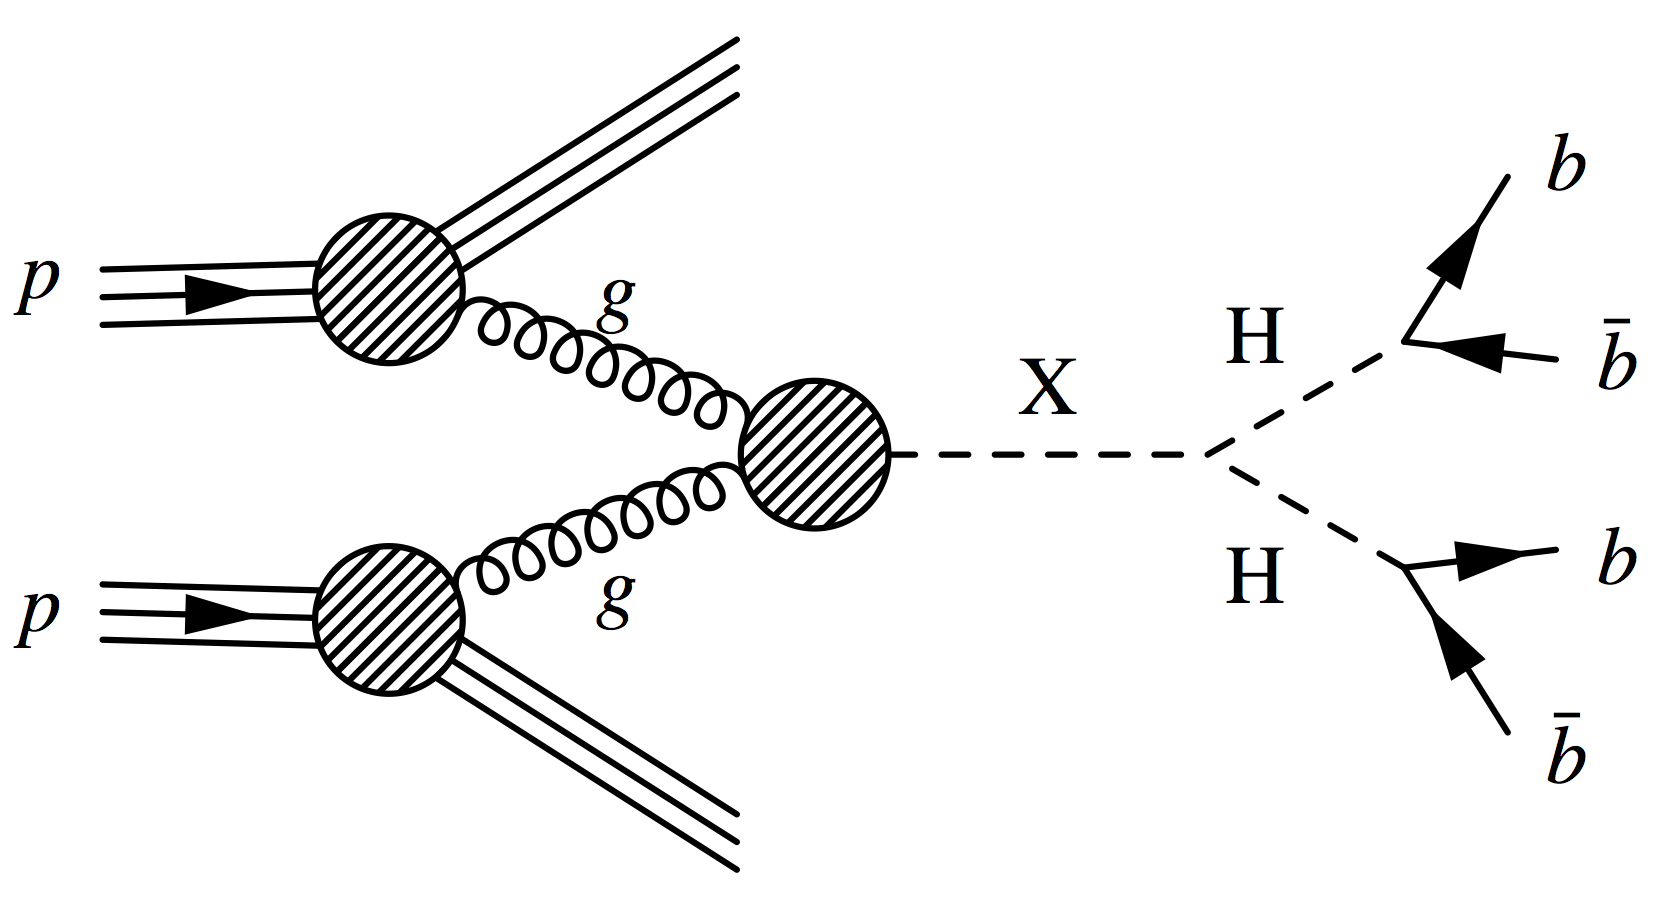
\includegraphics[width=0.4\linewidth]{feynman-diag-higgs.png}
    }
    \only<4>{
      \begin{block}{Difficulties}
      \begin{itemize}
        \item What exactly are the common features of the theories?
        \item What exactly is the state space we're describing?
        \item Divergent integrals, asymptotic ($\neq$ converging) series, \dots
      \end{itemize}
      \end{block}
    }
    \only<5|handout:0>{
      \begin{block}{Difficulties}
      \begin{itemize}
        \item Axioms.
        \item Describe measurements instead.
        \item Starting from the axioms, use formal mathematics, and allow flexibility elsewhere instead.
      \end{itemize}
      \end{block}
    }
  \end{overlayarea}
  \note[item]{Diagrams: \\ beta decay (mediated by weak force) \\ Higgs production}
  \note[item]<4- >{van Howe -> different ways of quantising give different theories for the same model}
  \note[item]<4- >{what are states? different pictures and unitary inequivalence, Haag's theorem}
\end{frame}

\begin{frame}[fragile]{Lie groups in Isabelle}
\note[item]{Some maths incoming - not so important for this talk.}
\begin{onlyenv}<1>
\begin{lstlisting}
locale lie_group =
  m_sqr: smooth_manifold_sqr charts +
  grp: group_on_with m_sqr.m1.carrier tms tms_one dvsn invs
  for charts::"('a::{t2_space, second_countable_topology},
                'e::euclidean_space) chart set"
    and tms tms_one dvsn invs +
  assumes smooth_mult:
      "diff \<infinity> m_sqr.prod_charts charts (\<lambda>(a,b). tms a b)"
    and smooth_inv:
      "diff \<infinity> charts charts invs"
\end{lstlisting}
\end{onlyenv}
\begin{onlyenv}<2|handout:0>
\begin{lstlisting}
locale lie_group =
  m_sqr: smooth_manifold_sqr charts +
  grp: group_on_with m_sqr.m1.carrier tms one +



  assumes smooth_mult:
      "diff \<infinity> (\<lambda>(a,b). tms a b)"
    and smooth_inv:
      "diff \<infinity> invs"
\end{lstlisting}
\end{onlyenv}
\end{frame}

\begin{frame}[fragile]{General Linear Group}
\newcommand{\GL}{\ensuremath{\text{GL}}}
\note[item]{}
\begin{overlayarea}{\textwidth}{0.5\textheight}
\begin{itemize}
  \item<1- > $\GL(n,\setR)$ is the group of all invertible $n\times n$ matrices.
  \item<3- > Elements of $\GL(n,\setR)$ represent linear operators on the vector space $\setR^n$.
  \item<4- > The homogeneous part of $\P$ is a subgroup of $\GL(4,\setR)$.
  \item<5-6> $\GL(n,\setR)$ is a Lie group! It is parametrised by real matrix elements\alt<5>{.}{\dots\\\vspace{10pt} \alert{But does the group structure agree with the continuous structure?}}
\end{itemize}
\end{overlayarea}
\vfill
\begin{overlayarea}{\textwidth}{0.3\textheight}
\begin{onlyenv}<2-3>
\begin{lstlisting}
abbreviation "GL \<equiv>
  {M::('a::comm_ring_1,'n::finite)square_matrix. invertible M}"
\end{lstlisting}
\end{onlyenv}
\begin{onlyenv}<4- >
\begin{lstlisting}
abbreviation "GL \<equiv> {M::('a,'n)square_matrix. invertible M}"
abbreviation GL\<^sub>R\<^sub>4::"(real,4)square_matrix set" where "GL\<^sub>R\<^sub>4 \<equiv> GL"
\end{lstlisting}
%abbreviation GL\<^sub>C\<^sub>4::"(complex,4)square_matrix set" where "GL\<^sub>C\<^sub>4 \<equiv> GL"
\end{onlyenv}
\end{overlayarea}
\end{frame}

\begin{frame}[fragile]{Transfer}
The \emph{transfer} package transfers theorems between related types. Say we want to transfer a result about a type $\alpha$ to $\beta$.
\vfill
\begin{minipage}{0.2\textwidth}
\begin{figure}
  \centering
  \begin{tikzcd}
    \alpha \arrow[d, "f"'] \arrow[r, "\cong"] & \beta \arrow[d, "g"] \\
    \alpha \arrow[r, "\cong"']                & \beta
  \end{tikzcd}
\end{figure}
\end{minipage}\hfill\pause
\begin{minipage}{0.7\textwidth}
\begin{itemize}[< +- >]
  \item $\alpha$ and $\beta$ \emph{related} by
    $\;\cong \colon \alpha \to \beta \to \texttt{bool}$
  \item prove $g$ maps related $f$-inputs to related $f$-outputs
  \item prove similar \emph{transfer rules} for all constants \\
    in the theorem to be transferred
  \item relations can be constructed from the type of a constant
\end{itemize}
  \note[item]<4- >{And then it works! It works both ways too.}
  \note[item]<5- >{This is the great contribution of transfer: generic construction for rules, and automation.}
  \note[item]{}
\end{minipage}
\end{frame}


\begin{frame}[fragile]\frametitle{WLOG for interval endpoints}
	Proofs mirror the structure of the preceding lemma.
	\setbeamercovered{transparent}
	\begin{enumerate}
	\item<2> State the desired result
	%\item This gives the symmetric proposition \lstinline|P| from the lemma
	\item<3> Split up the proof into essentially distinct cases with fixed events
	\end{enumerate}
	\setbeamercovered{invisible}
{\lstset{escapeinside=||}
\begin{lstlisting}
let ?prop = "\<lambda> I J. is_int (I\<inter>J) \<or> (I\<inter>J) = {}"
{ fix I J a b c d
  assume "I = interval a b" "J = interval c d"
  { assume "betw4 a b c d"
    have "I\<inter>J = {}" (*...*)
  } { assume "betw4 a c b d"
    have "I\<inter>J = interval c b" (*...*)
  } { assume "betw4 a c d b"
    have "I\<inter>J = interval c d" (*...*)
  } }
|\tmark{}|then show "is_int (I1\<inter>I2)"
  using wlog_interval_endpoints_distinct symmetry|\tmark{}| assms
  by simp
\end{lstlisting}}
\makehl{1}{2}
\end{frame}

\end{document}